\documentclass[12pt]{article}
\usepackage[english]{babel}
\usepackage[utf8x]{inputenc}
\usepackage{amsmath}
\usepackage{tikz}
\usetikzlibrary{arrows,automata}
\begin{document}
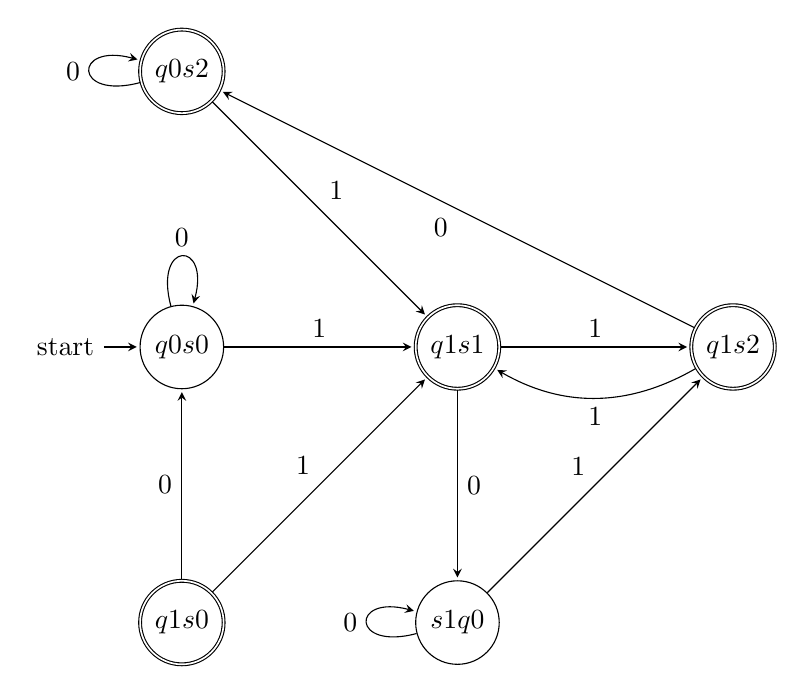
\begin{tikzpicture}[->,>=stealth,shorten >=1pt,auto,node distance=3.5cm,scale = 1,transform shape]
\node[state,initial] (q0s0) {$q0s0$};
\node[state,accepting] [below of=q0s0](q1s0) {$q1s0$};
\node[state] [right of=q1s0](s1q0) {$s1q0$};
\node[state,accepting] [right of=q0s0](q1s1) {$q1s1$};
\node[state,accepting] [above of=q0s0](q0s2) {$q0s2$};
\node[state,accepting] [right of=q1s1](q1s2) {$q1s2$};
\path (q0s0)	edge	[loop above]	node{$0$} (q0s0)
(q0s0)	edge		node{$1$} (q1s1)
(q1s0)	edge		node{$0$} (q0s0)
(q1s0)	edge		node{$1$} (q1s1)
(s1q0)	edge	[loop left]	node{$0$} (s1q0)
(s1q0)	edge		node{$1$} (q1s2)
(q1s1)	edge		node{$0$} (s1q0)
(q1s1)	edge		node{$1$} (q1s2)
(q0s2)	edge	[loop left]	node{$0$} (q0s2)
(q0s2)	edge		node{$1$} (q1s1)
(q1s2)	edge		node{$0$} (q0s2)
(q1s2)	edge	[bend left]	node{$1$} (q1s1)
;\end{tikzpicture}
\end{document}